\chapter{Conclusiones}
\section{Aportaciones}
\label{sec:org455dd2e}
Al partir de un proyecto ya creado, \texttt{solaR}, surge la necesidad de explicar cuáles son las aportaciones de este paquete. Para ello, se puede usar el repositorio donde se ha alojado este proyecto y comentar los datos que este ofrece.

\subsection{Blame}
\label{sec:orged9c22b}
En GitHub, el término \emph{blame} se refiere a una función que permite ver quién fue el autor de cada línea específica de código en un archivo. Por ejemplo, si se quisiera ver quién ha realizado cada línea de la función \texttt{fCompD} en GitHub, se podría acceder a su página en el repositorio, y pulsar en el botón \href{https://github.com/solarization/solaR2/blame/master/R/fCompD.R}{\emph{blame}}.

Una vez en esta pestaña (figura \ref{fig:blame}), se pueden distinguir varias partes:
\begin{figure}[htbp]
\centering
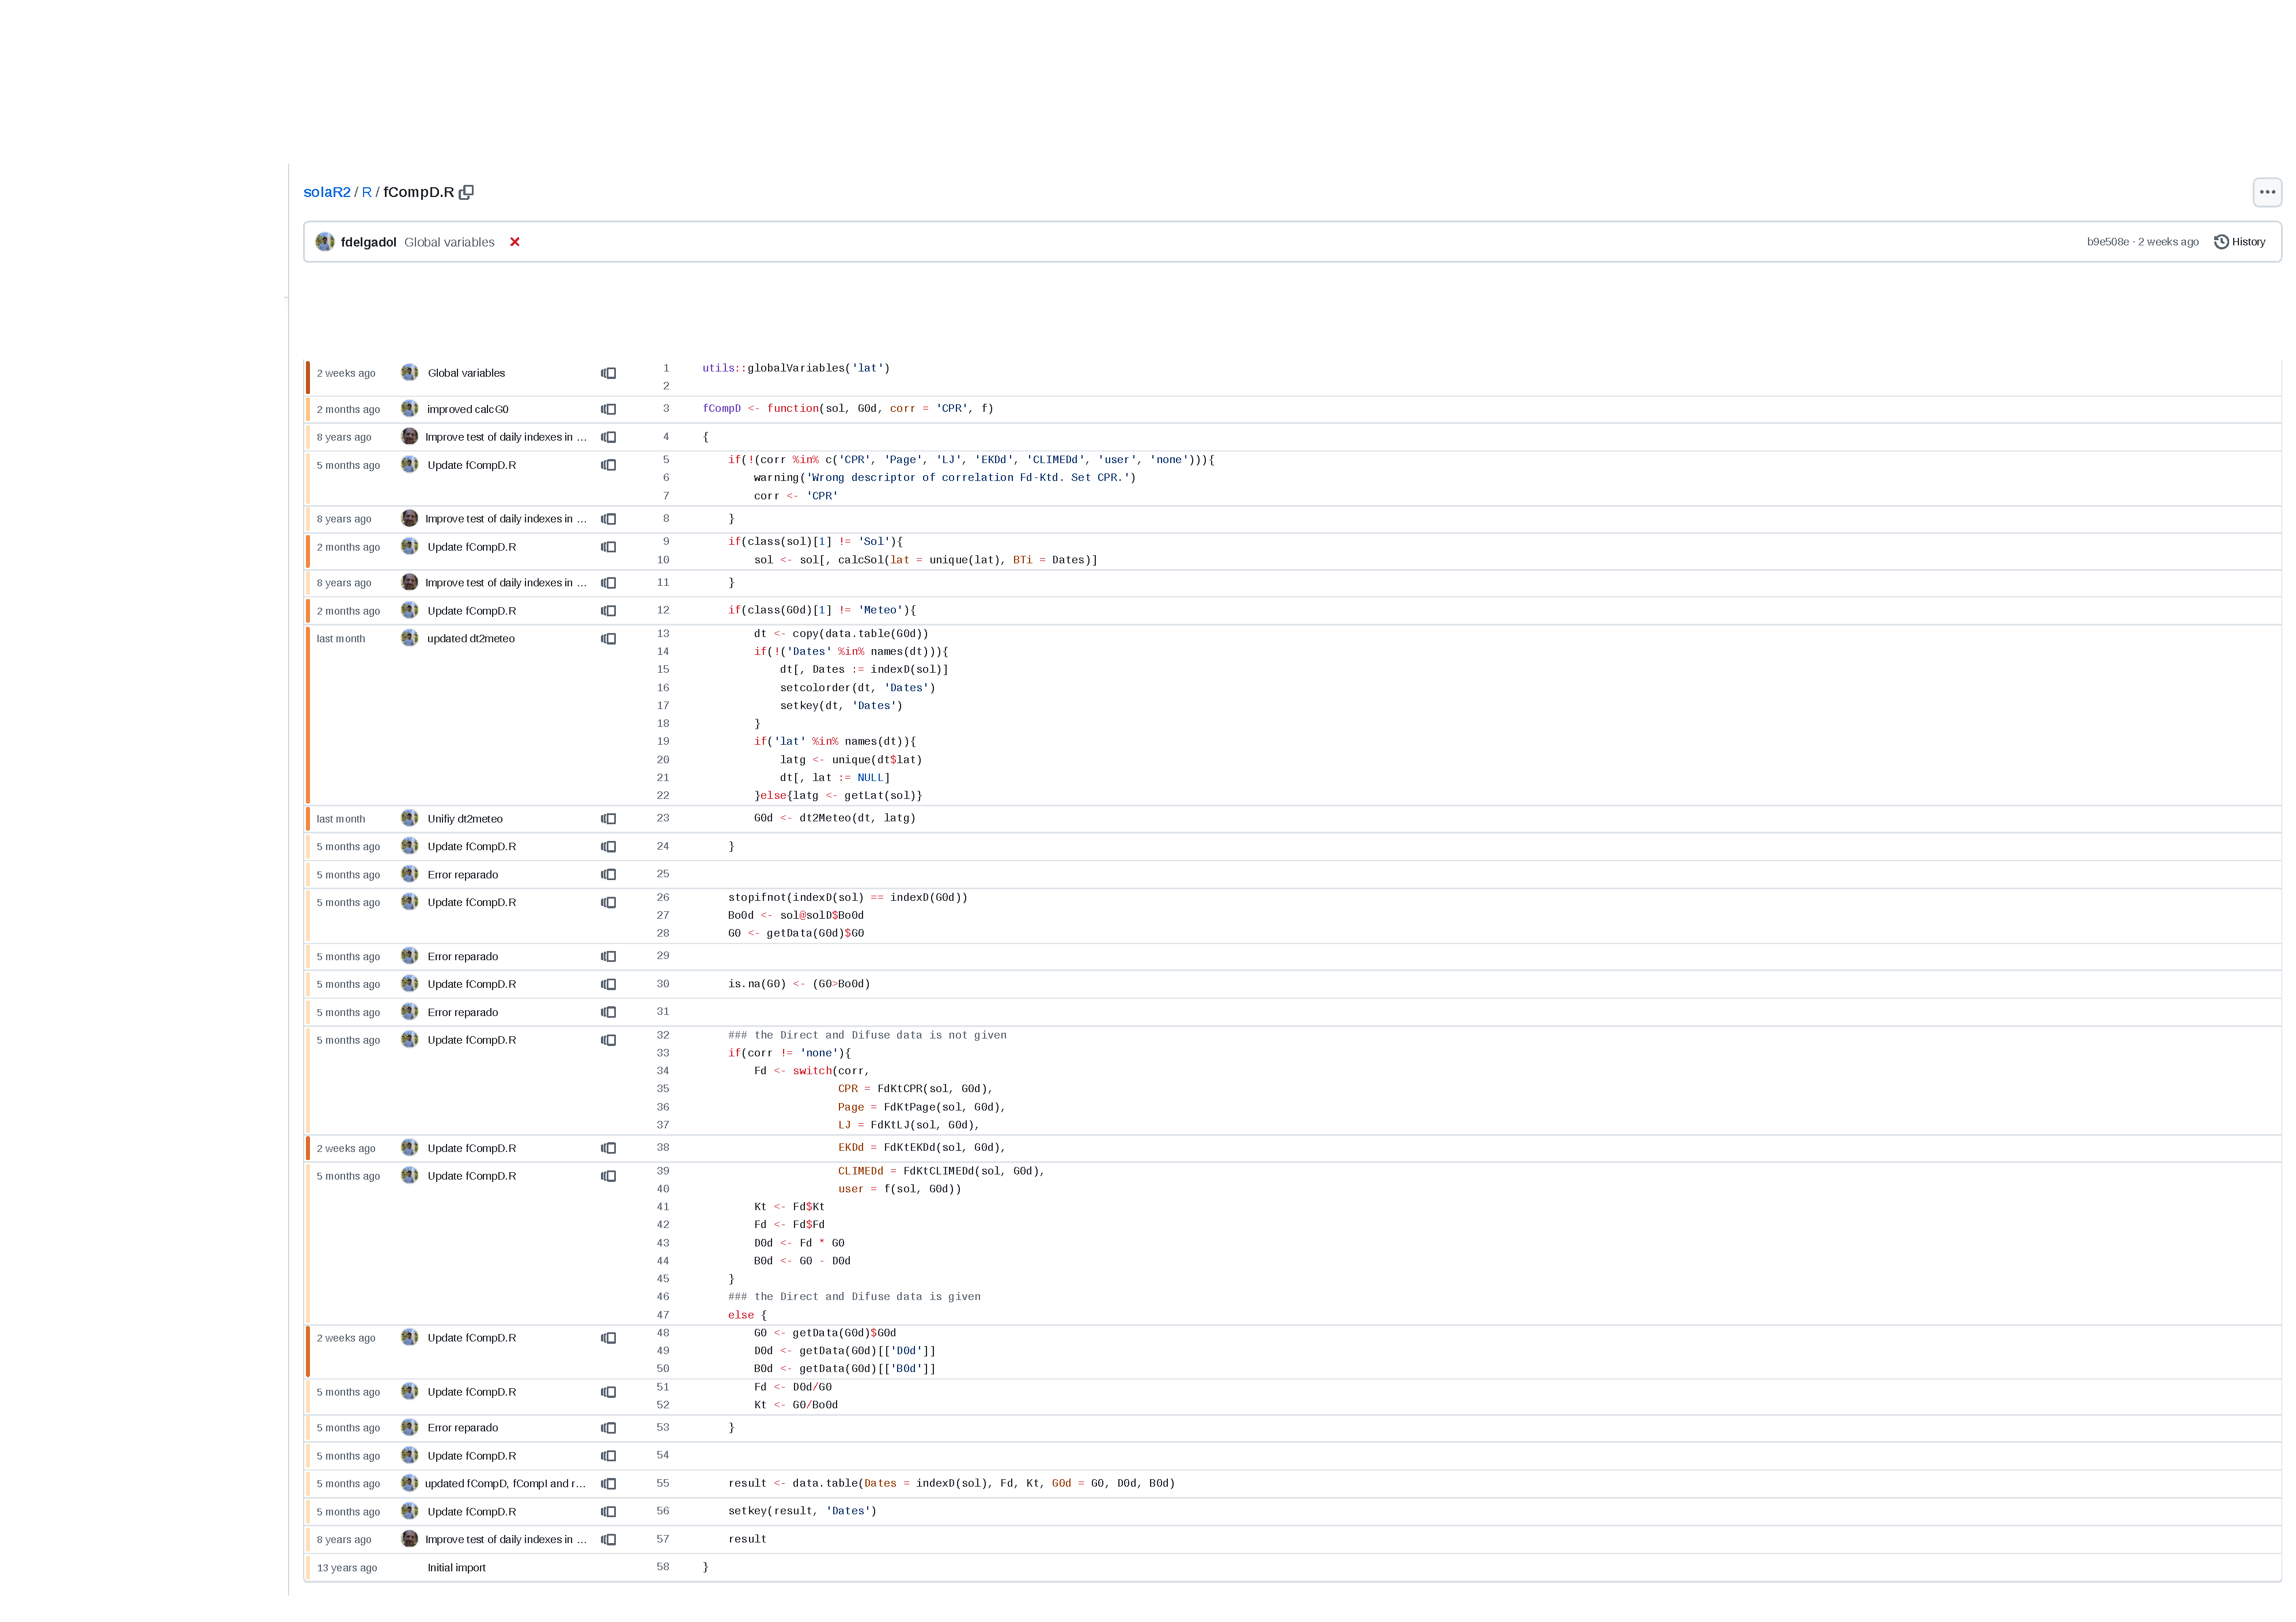
\includegraphics[width=.9\linewidth]{figuras/blame-fCompD.pdf}
\caption{Pestaña \emph{blame} de GitHub de la función \texttt{fCompD}. \label{fig:blame}}
\end{figure}
\begin{itemize}
\item A la izquierda, se puede ver la fecha en la que se modificó esa línea por última vez.
\item A continuación, se tiene el nombre del \emph{commit}\footnote{Un \emph{commit} es una operación que guarda los cambios realizados en el repositorio. Funciona como un punto de control en el historial del proyecto.} en el que se cambió.
\item Después, se puede tener acceso al \emph{blame prior}, en el cual se puede ver cómo era el resto del archivo cuando se realizó ese \emph{commit}.
\item Por último, se muestra el número de línea y su contenido.
\end{itemize}

Este análisis resulta revelador a la hora de comprender los aportes de este proyecto, ya que se pueden entender los cambios que se han hecho y comprenderlos en el contexto de cada momento del proyecto.

\subsection{Insights}
\label{sec:orgcb7a18e}
GitHub también cuenta con una serie de herramientas y características que proporcionan información detallada y análisis sobre el rendimiento, la actividad y la salud de un repositorio. Entre ellas, se encuentra \emph{contributors}. Esta herramienta muestra información sobre las contribuciones individuales de los miembros del equipo. Con ella, se puede ver el número de líneas añadidas y eliminadas y el número de \emph{commits} realizado por cada miembro (\ref{fig:contributors}).
\begin{figure}[htbp]
\centering
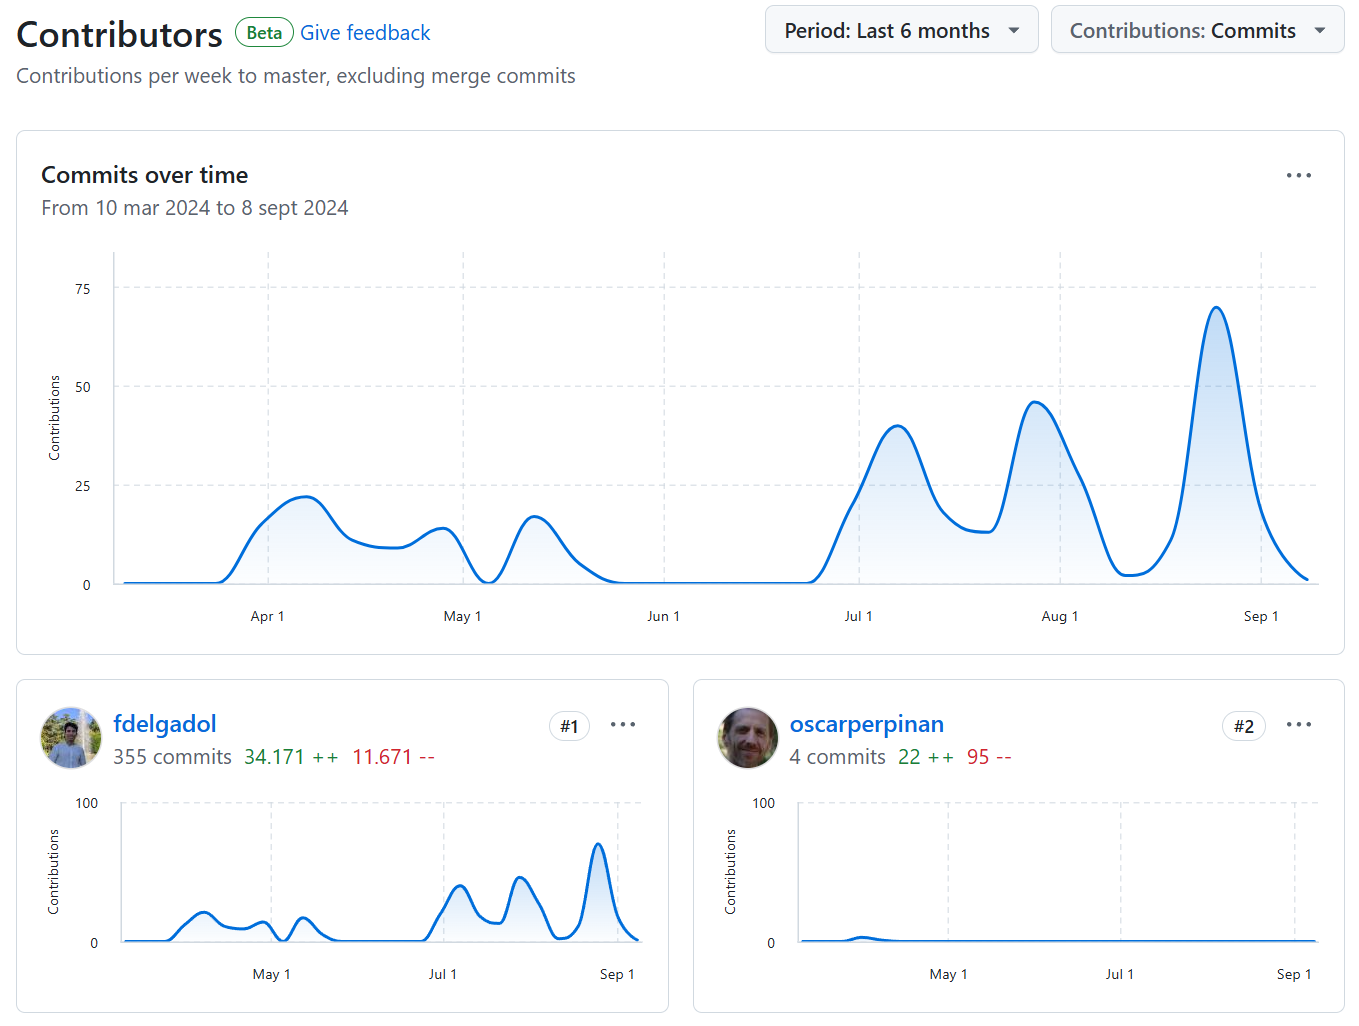
\includegraphics[width=.9\linewidth]{figuras/contributors.png}
\caption{Sección \emph{contributors} de GitHub para los últimos 6 meses. \label{fig:contributors}}
\end{figure}

Todas estas herramientas dejan ver la magnitud de los cambios que se han producido en este proyecto en comparación con el anterior.

\section{Comparación de resultados}
\label{sec:orgbee4992}
Como se ve en el capítulo \ref{chap:ejemplo-practico-aplicacion}, los resultados son identicos a los que ofrecía \texttt{solaR}. Sin embargo, el número de funciones es mayor, lo que permite calcular datos aislados facilitando mucho las labores de investigación. Además, los tiempos de ejecución y el uso de memoria han disminuido mucho.
\begin{lstlisting}[numbers=left,language=r,label= ,caption= ,captionpos=b]
lat <- 37.2;

G0dm <- c(2766, 3491, 4494, 5912, 6989, 7742, 7919, 7027, 5369, 3562,
          2814, 2179)

Ta <- c(10, 14.1, 15.6, 17.2, 19.3, 21.2, 28.4, 29.9, 24.3, 18.2,
        17.2, 15.2)

prom <- list(G0dm = G0dm, Ta = Ta)

profvis({prodFixed <- prodGCPV(lat = lat, dataRad = prom,
                      keep.night = FALSE)})
\end{lstlisting}

\begin{figure}[h!]
  \centering
    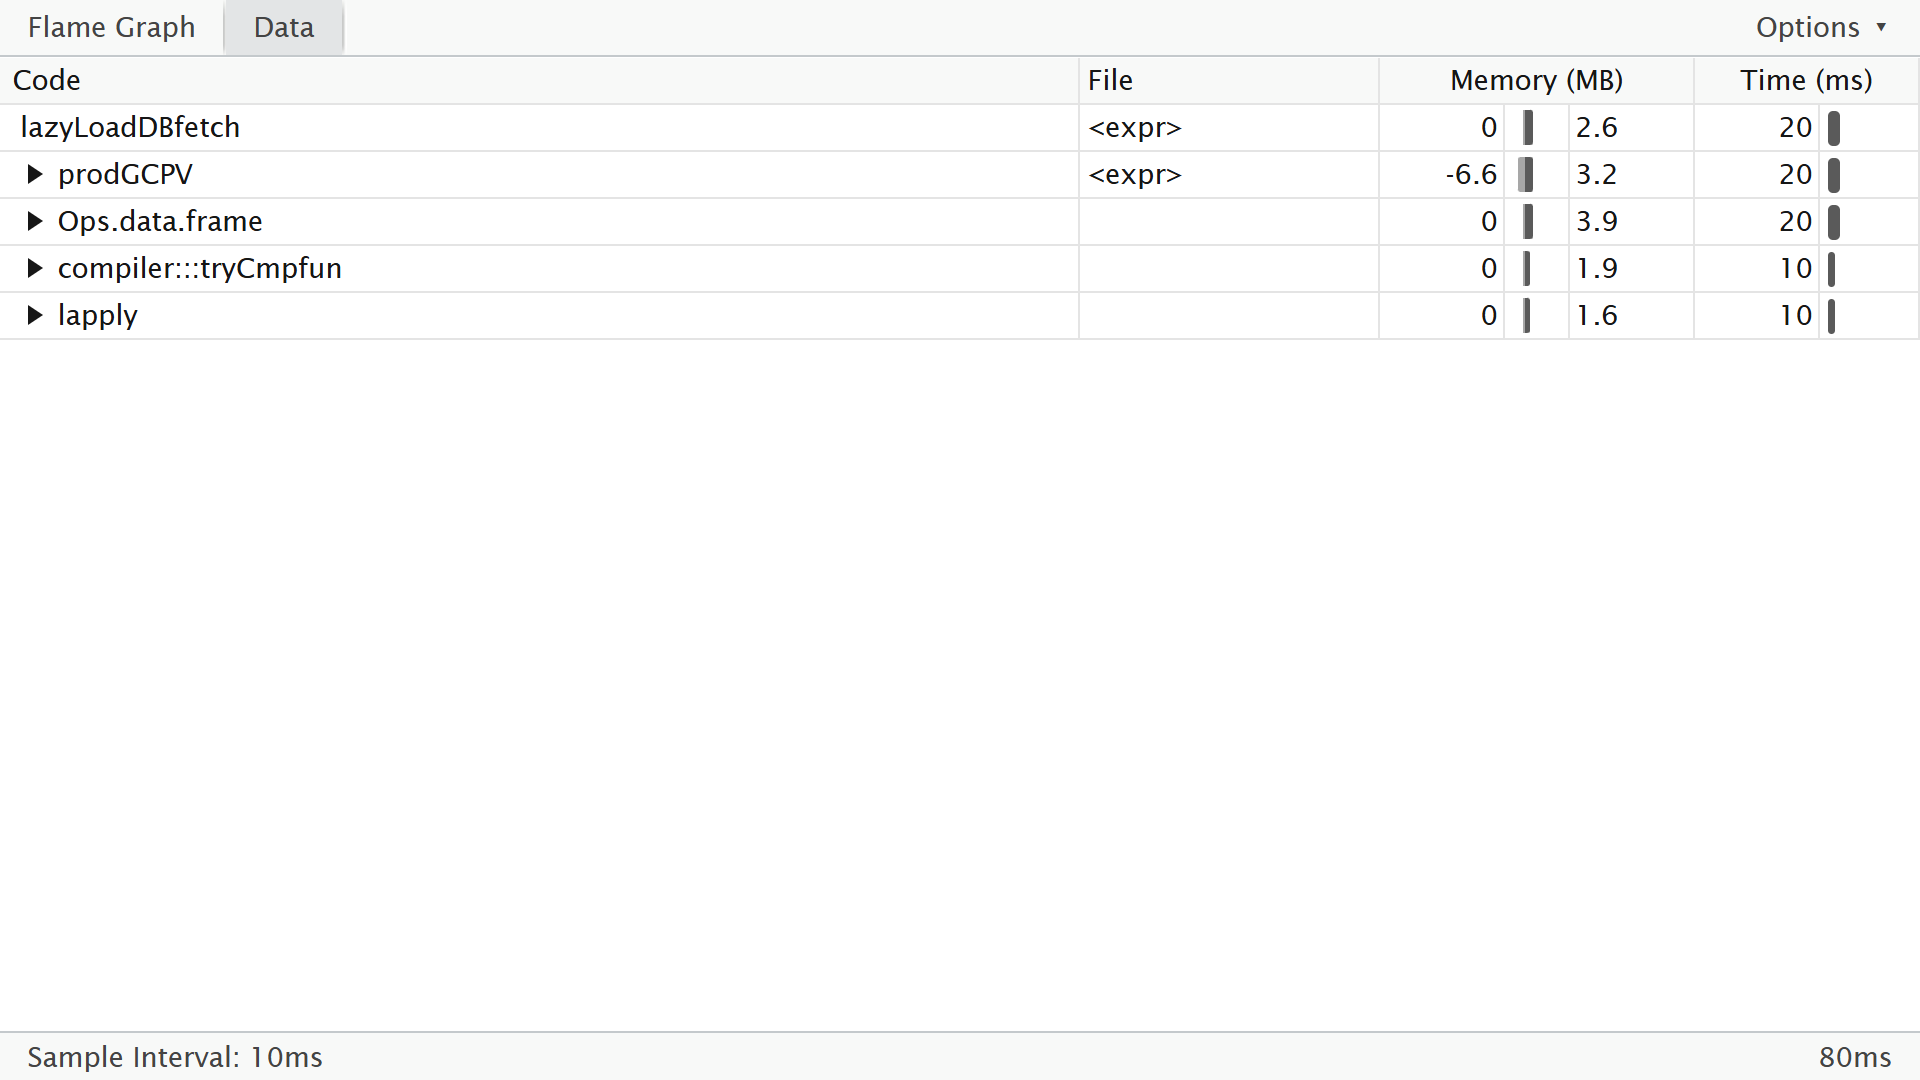
\includegraphics[width=\textwidth]{figuras/data.png}
    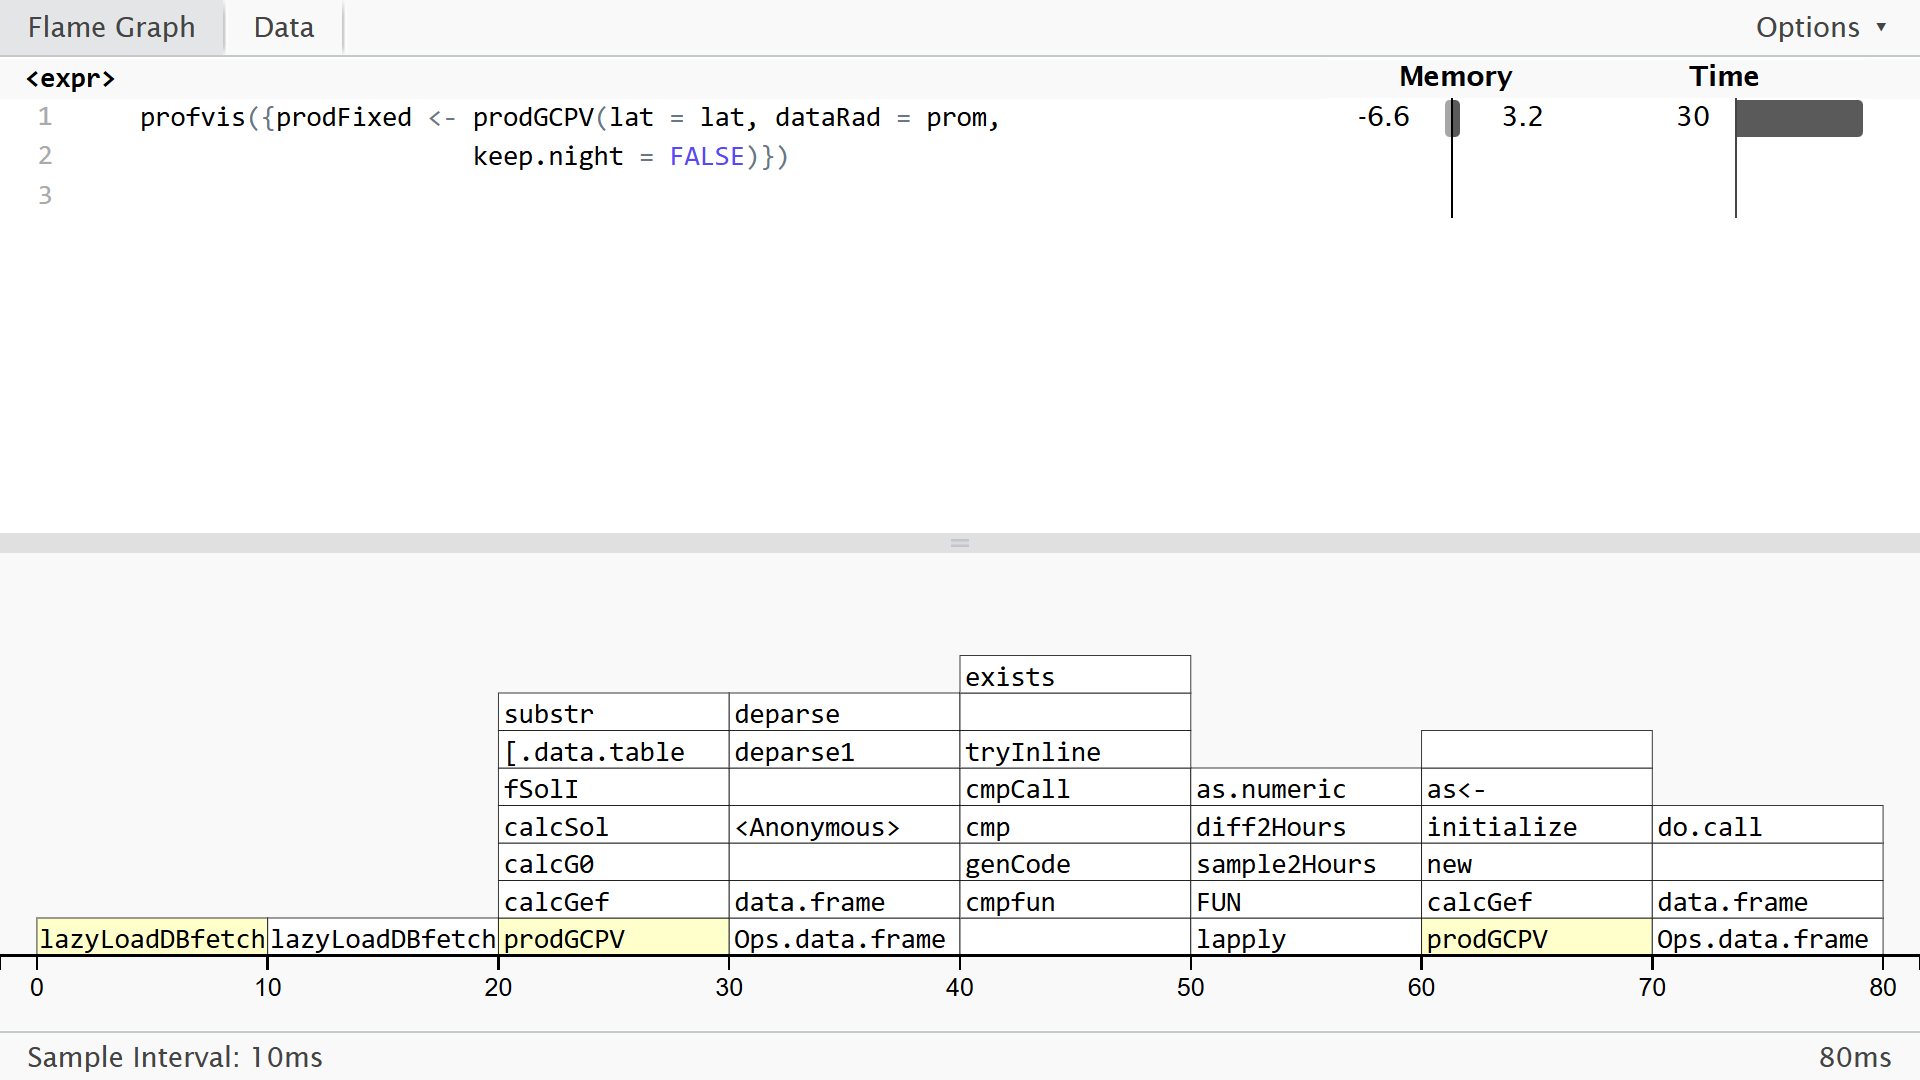
\includegraphics[width=\textwidth]{figuras/flamegraph.png}
  \caption{Resultado de rendimiento de la función \texttt{prodGCPV} obtenidos con la función \texttt{profvis}. Arriba, la pestaña \textit{Data}; y abajo, la pestaña \textit{Flame Graph}}
\end{figure}

\FloatBarrier

\section{Desarrollo futuro}
\label{sec:org29b2c12}
Pese a que \texttt{solaR2} ya es un paquete muy capaz, aún quedan varios puntos a mejorar:
\begin{itemize}
\item \textbf{Interfaz de usuario}: el lenguaje \texttt{R} es un lenguaje orientado a objetos, por lo que un paquete basado en este, puede entorpecer a los usuarios menos entendidos en este lenguaje. Por ello, cabe la posibilidad de añadir al paquete una interfaz de usuario que permita a los usuarios introducir sus datos de forma guiada.
\item \textbf{Mejora de funciones}: muchas funciones pueden seguir desarrollándose, mejorando su eficiencia o simplemente incluyendo nuevas funcionalidades.
\item \textbf{Toma de datos}: Aunque \texttt{solaR2} ya cuente con la función \texttt{readSIAR}, mejoraría notablemente incorporando una función que sea capaz de obtener datos meteorológicos de forma ilimitada (la función \texttt{readSIAR} tiene un límite de 100 registros por minuto).
\item \textbf{Uso de paquetes especializados en datos espaciales}: Paquetes como \texttt{terra} \cite{hijmans24} podrían ser útiles para aumentar la eficiencia y rapidez de \texttt{solaR2}.
\end{itemize}
